\subsection{Fix particles}
\label{sss:aquagpusph:boundaries:fixparticles}
%
`Fix particles', also called `dummy particles' sometimes, is a extension of the fluid domain along walls with a little
bit especial fluid particles linked to them.\\
%
In figure \ref{fig:aquagpusph:FixParticlesScheme} an scheme of the fixed particles distribution is shown. Must be
noticed that first row of fixed particles is placed \textit{dr}/2 inner on wall, and the several rows are placed
every \textit{dr}. The fixed particles are similar to the fluid ones, but a normal must be provided and
\textit{imove} flag must be lower than 0.\\
%
The fixed particles will use continuity equation like the fluid particles, but not momentum equation, because
fixed particles velocity is linked to the wall motion. Related to this, if no motions are set, the initial fixed
particles velocity will be preserved along the simulation\footnote{you can modify this behaviour with custom
predictor and corrector kernels}.\\
%
SPH equations when `Fix particles' boundary condition is used are therefore
%
\[
\left. \left\langle \frac{\gradient p}{\rho} \right\rangle_a \right\vert_{a \in \mathrm{Fluid}} = \frac{1}{\gamma_a}
	\sum\limits_{b \in \mathrm{Fluid}\;\cup\;\mathrm{Boundary}} 
		\left( \frac{p_a}{\rho_a^2} + \frac{p_b}{\rho_b^2} \right)
	\gradient W_{ab} m_b
\]
%
\[
\left. \left\langle \rho \; \divergence(v) \right\rangle_a \right\vert_{a \in \mathrm{Fluid}\;\cup\;\mathrm{Boundary}} =
	- \frac{1}{\gamma_a}
	\sum\limits_{b \in \mathrm{Fluid}\;\cup\;\mathrm{Boundary}} 
		\left( v_a - v_b \right)
	\gradient W_{ab} m_b
\]
%
\[
v_{a \in \mathrm{Boundary}} = \mathrm{f}\left(x_\mathrm{walls} \left( t \right) \right)
\]
%
Where $\gamma_a$ can be forced to be 1 ever setting Shepard correction to ``None'' as decribed on the chapter
\ref{sss:XML:SPH}, that have the advantage of getting a fully conservative notation.\\
%
`Fix particles' uses internally `ElasticBounce boundary' condition described on section
\ref{sss:aquagpusph:boundaries:elasticbounce}. It's strongly recommended let `Fix particles' work with
`ElasticBounce boundary' in order to warranty that the particles can trespass the walls, but if you want to
disable this feature simply set `BoundDist' parameter to 0, \textbf{never pass null normals to the fixed
particles}.\\
%
`Fix particles' is chronologically the first boundary condition implemented on SPH, has the main advantage that is
easy to implement since the fixed particles have a really similar treatment to the usual fluid particles, but
have the main disadvantage of the particles velocity set using only walls motion as a `U0M', that gives an
inconsistent Laplacian operator. Also requires increase the number of particles significantly, more as the number of neighbours grows.
%
\begin{figure}[ht!]
  \centering
  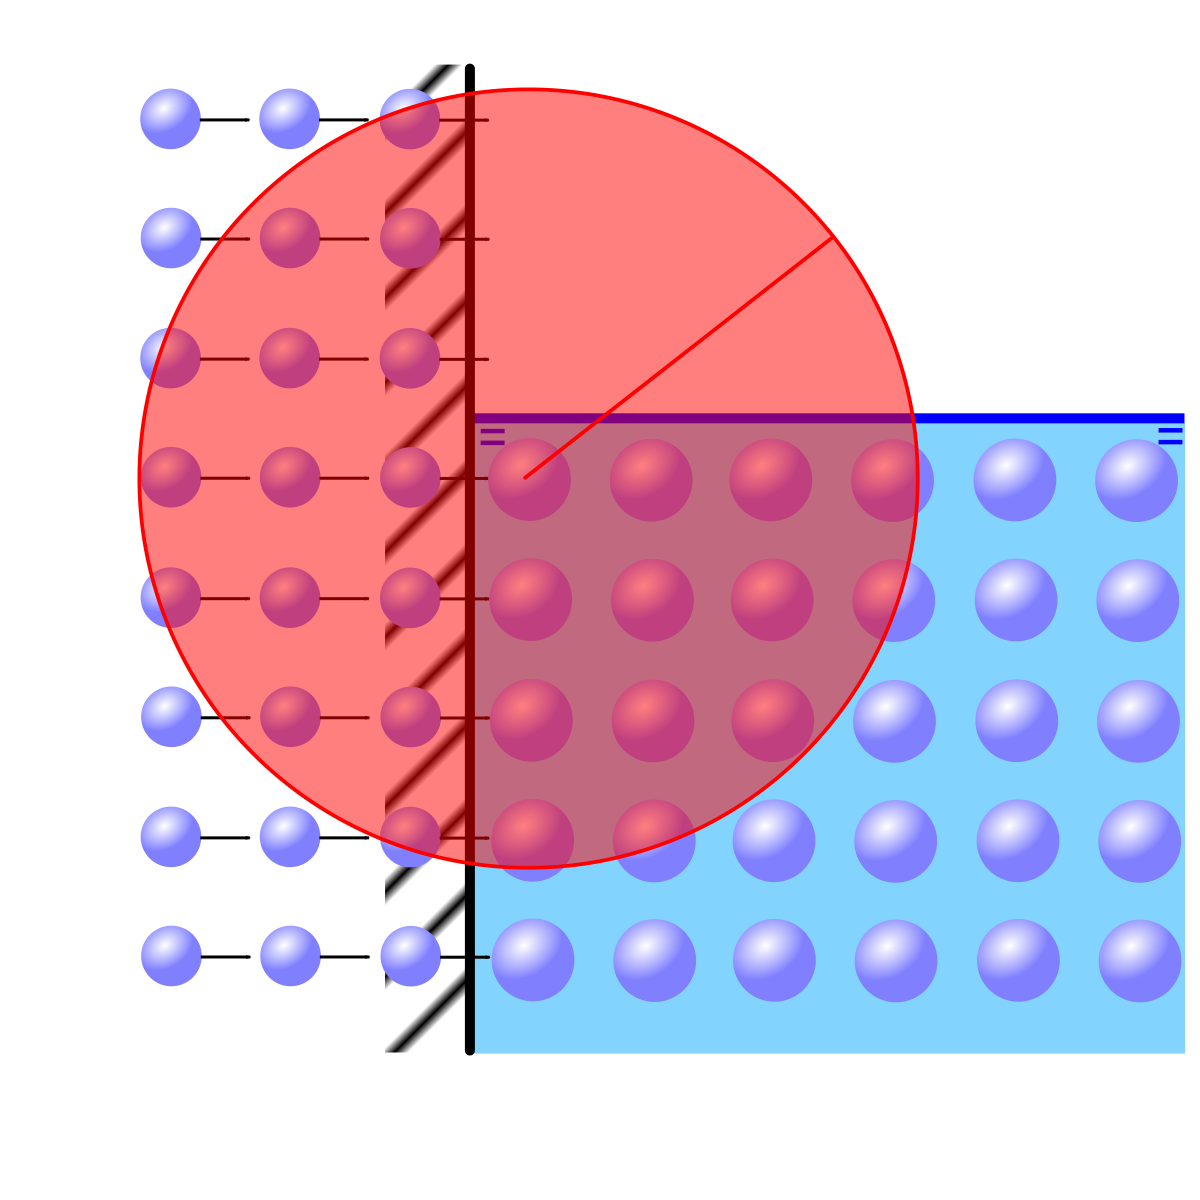
\includegraphics[width=0.4\textwidth]{FixedParticles}
  \caption{Fix particles scheme}
  \label{fig:aquagpusph:FixParticlesScheme}
\end{figure}
%